\documentclass{article}
\usepackage[utf8]{inputenc}
\usepackage[%
  style=numeric, 
  sortcites,
  backend=biber,
  giveninits=true % <===================================================
]{biblatex}
\usepackage{graphicx}
\usepackage{float}


\addbibresource{papers.bib}


\date{February 14 2020}

\author{
  Chia-Wei Chen\\
  \texttt{cchen562@wisc.edu}
  \and
  Yu-Huai Chen\\
  \texttt{ychen874@wisc.edu}
  \and
  Chung-Shien Luh\\
  \texttt{luh@wisc.edu}
}
\title{
Image-based Virtual Try-on Generator\\
\large CS766 Computer Vision Project Proposal
}

\begin{document}

\maketitle

\section{Problem Statement}

In this project, we will focus on the evolution of the virtual try-on systems using images of clothes on the Internet and photos of models from e-commerce websites. We will divide developments of the project into three stages. First, we focus on investigating methods with traditional computer vision techniques that we have learned in class such as image stitching and will analyze meaningful insights and trade-off within these approaches. In the second stage, we will turn our attention to the recent deep learning techniques in the virtual try-on application. For example, using generative adversarial nets (GAN) \cite{goodfellow2014generative} as a generative machine learning model to synthesize virtual image of the model wearing some unseen clothes. Finally, we will implement the current state-of-the-art virtual try-on algorithm from top-tier research publications and evaluate its reproduciblility.


\section{Motivation}

\begin{figure}[h]
    \centering
    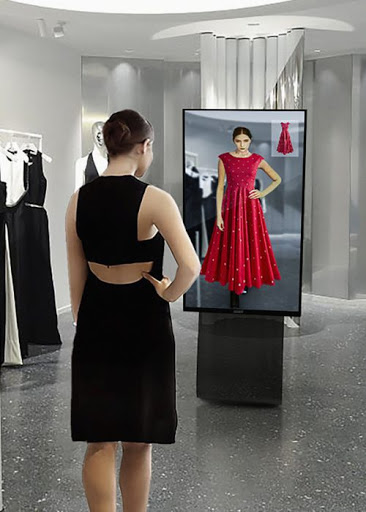
\includegraphics[width=0.3\textwidth]{fit-ar.jpg}
    \caption{Virtual Dressing Room \cite{vdr}}
\end{figure}

Nowadays, people are purchasing most of their items online and are spending more on it especially in fashion items since browsing different styles and categories of clothes is easy with just a few mouse clicks. Despite the convenience that online shopping provides, customers tend to concern about how a particular fashion item image on the website would fit with themselves. Therefore, there is an urgent demand to provide a quick and simple solution for virtual try-on. Instead of using 3D information such as depth of the image, we believe simply rely on the regular 2D photo is the most convenient way to satisfy this need. With the recent progress in virtual try-on technologies, people can have a better online shopping experience by accurately envisioning themselves wearing the clothes from online categories. Furthermore, virtual try-on technologies not only have demand in online shopping but also in physical shopping. In other words, with the try-on technologies developed on mobile application, customers can save their time of going into the fitting room.

\section{Background}

Seminal work on virtual fitting with traditional computer vision techniques is DRAPE \cite{guan2012drape}. DRAPE model is trained with meshes of pose of person and shapes of clothes. They utilized \textit{shape deformation gradients}, a linear transformation function that aims to align triangles from source and target mesh, to represent deformation between meshes. DRAPE applied the process of deformation due to body shape, rigid part rotation, and body pose. Recent advances in machine learning, in particular, deep neural networks forwards the performance of virtual try-on systems significantly. VITON \cite{han2018viton} is a virtual try-on network with an encoder-decoder generator as its core component. Instead of accessing 3D information such as in previous techniques \cite{guan2012drape}, VITON only leveraged 2D information in its virtual try-on network. Therefore, VITON reduces the resource footprint and enables a broader set of applications. State-of-art methods such as ClothFlow \cite{han2019clothflow} outperforms VITON by extending the networks in VITON. In particular, ClothFlow divides the try-on framework into three stages. (1) target segmentation map generation. (2) refinement of geometric information in a cascaded warping manner. (3) synthesis of the final result. These extra stages are shown to improve the synthesis of photo-realistic images. 

\section{Evaluation}

We will apply the same evaluation methods described by Han et al in \cite{han2018viton}. In particular, we will use the VITON dataset we found online and we will measure the inception score for both traditional techniques and deep learning approach proposed in VITON.
Inception score is usually used to quantitatively evaluate the synthesis quality of image generation models. Higher inception scores indicate the evaluated model can produce visually diverse and semantically meaningful images which demonstrates the generality of a given machine learning approach. 

\section{Deliverables \& Milestones}
We will write some code and run some experiments.

Our plan is to start by investigating traditional computer vision methods such as image stitching we learned in class and papers such as DRAPE \cite{guan2012drape} and gradually move onto newer approaches such as deep learning-based techniques. We will try to use pre-trained model if provided for each methods before we try to re-implement the best or current state-of-the-art method.

% dax go go go
% dax zZZ zZZ
% 739 做實驗
\begin{itemize}
    \item 2/21: Read and research some more papers. Create a webpage or a shared media for documenting the project.
    \item 3/13: Finish investigations for traditional CV (DRAPE) vs. VITON / VITON-GAN vs. ClothFlow.
    \item 3/20: Start some re-implementation of state-of-the-art paper.
    \item 3/25: Finish Project Mid-Term Report.
    \item 4/10: Finish re-implementation and start evaluation and comparison for different datasets (VITON vs DeepFashion). Find ways to improve existing solutions.
    \item 4/27, 4/29, or 5/1: Wrap-up and finish slides for Final Project Presentations
    \item 5/4: Finish Project Webpage.
\end{itemize}

\section{E-Dressing}
We investigated E-Dressing \footnote{\url{https://github.com/iamsusmitha/E-Dressing}} which is a system that uses traditional machine learning methods, in particular, an ensemble of regression trees \cite{kazemi2014one}, to perform the tasks of virtual try-on. However, after experimenting with the system and running author-provided demos, we would argue that E-Dressing is limited to try-on of items on faces. For example, glasses and earrings. Although this does not align with our original plan of the project, we see the possibility of integrating this feature into our final system to have a full-body try-on feature since CP-VTON (as described below) only support try-on of shirts. 


\section{CP-VTON}
We've reimplemented the paper (Toward Characteristic-Preserving Image-based Virtual Try-On Network) method using the same dataset and settings.

\subsection{Dataset \& Preprocessing}
For the dataset, we use the same data provided by original VITON \& CP-VTON \cite{viton-data}, which use OpenPose\cite{cao2018openpose} for JSON format pose information, and LIP\_JPPNet\cite{liang2018look} for model image segmentation.

\subsection{Methodology}
In CP-VTON, they use a two-stage solution to deal with the virtual try-on problem. First, it learns a transformation for transforming the clothes into fitting the body shape of the target person via a new Geometric Matching Module (GMM). Second, to mitigate edge artifacts of warped clothes and make the results more realistic, CP-VTOM applies a Try-On Module (TOM) that learns a combination mask to integrate the warped clothes and the  rendered image to ensure smoothness.
\subsubsection{Geometric Matching Module (GMM)}
    \begin{itemize}
        \item input: Person Representation p (Keypoints + Segmentation + Human Model Image) + Cloth c (In-shop Clothes)
        \item output: Warped Clothes
        \item loss function: $L_{1}$ loss
    \end{itemize}
\subsubsection{Try-On Module (TOM)}
    \begin{itemize}
        \item input: Person Representation p (Keypoints + Segmentation + Human Model Image) + Warped Clothes c' (generated by GMM)
        \item output: Human Model with warped cloth
        \item loss function: $L_{1}$  + $L_{VGG}$ loss
    \end{itemize}

\subsection{Evaluation}
Train and test model mentioned in the original paper (put metric and image and visualize). Furthermore, we use our own data (Cloth + Human Model Image) to see the model effect.

\begin{figure}[h]
    \centering
    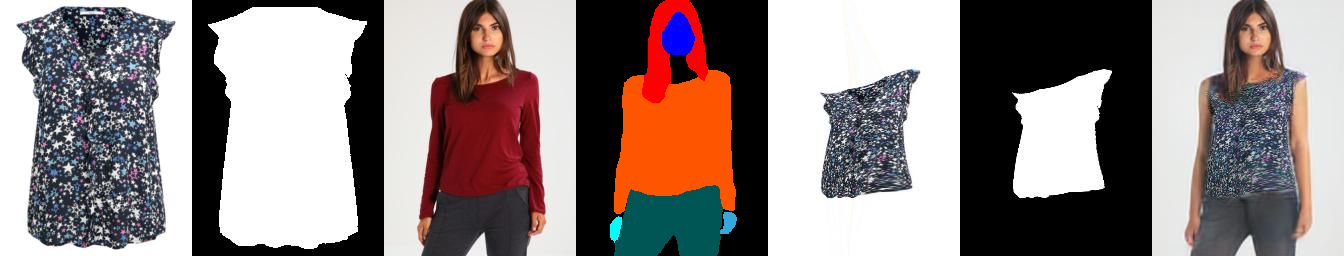
\includegraphics[width=1\textwidth]{cp-vton-imgs/visual1.png}
    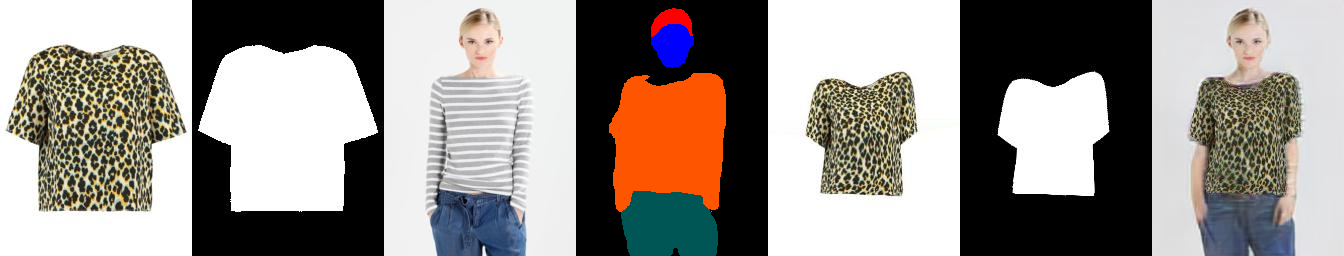
\includegraphics[width=1\textwidth]{cp-vton-imgs/visual2.png}
    \caption{Visualization of cp-vton \cite{vdr}}
\end{figure}



\printbibliography
\end{document}
